\chapter{Analyse}
\graphicspath{ {./images/} }

\section{Insertion}

\begin{figure}[H]
    \centering
    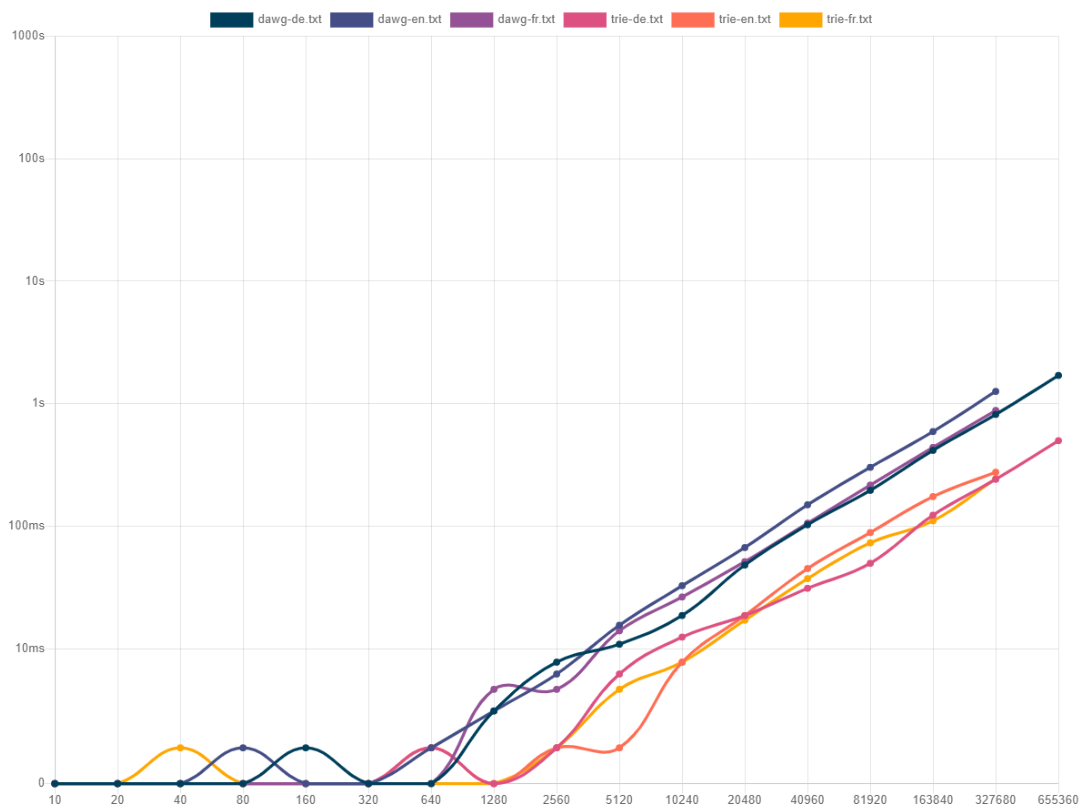
\includegraphics[scale=0.5]{images/time_insert.png}
    \caption{\label{HomePage} Temps d'insertion}
\end{figure}

On rappelle que, en théorie :
\begin{itemize}
  \item[-] Trie : O(L * log(n)) avec L la longueur maximale d'un mot et n le nombre de mots
  \item[-] Dawg : O(log(n)) avec n le nombre d'état dans le dictionnaire.
\end{itemize} \leavevmode

En pratique : \medskip \newline
L'insertion dans les deux structures semble être de même complexité, même si l'insertion dans un Trie prend environ deux fois moins de temps que dans un Dawg.\newline Ce qui est normal car il faut minimiser la structure Dawg à chaque insertion.

\section{Recherche}

\begin{figure}[H]
    \centering
    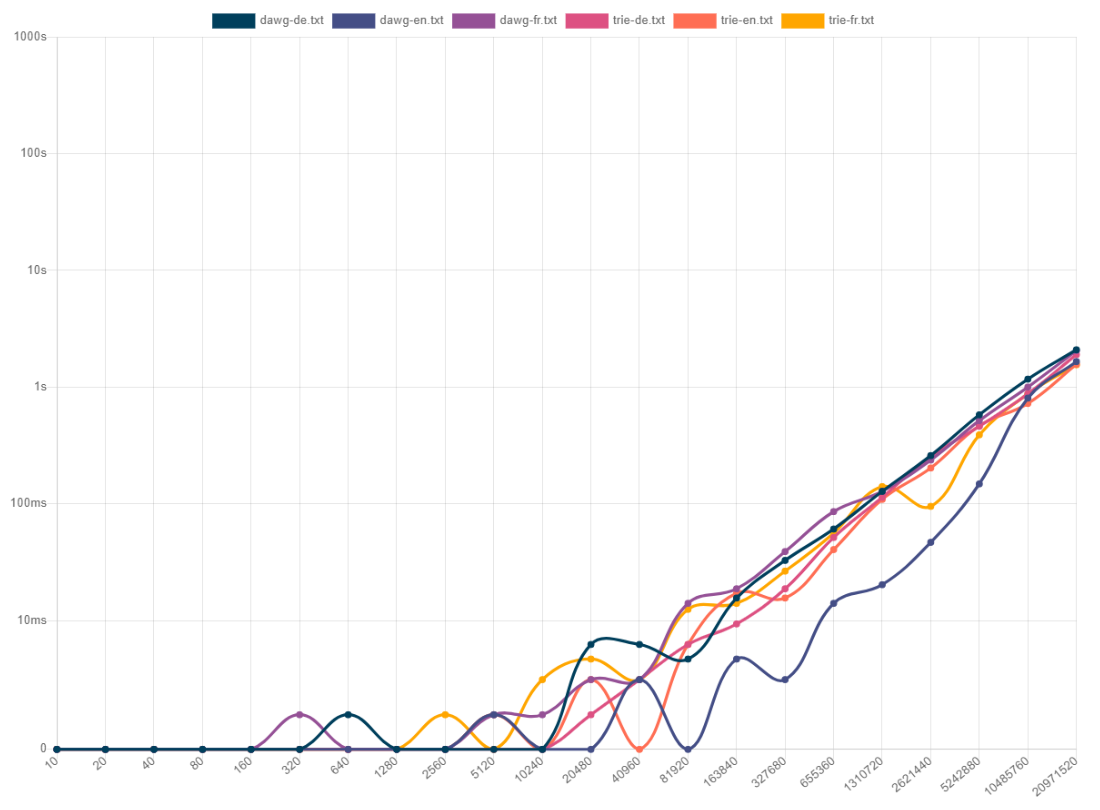
\includegraphics[scale=0.5]{images/time_search.png}
    \caption{\label{HomePage} Temps de recherche}
\end{figure}

On rappelle que, en théorie :
\begin{itemize}
  \item[-] Trie : O(L) avec L la longueur maximale d'un mot.
  \item[-] Dawg : O(log(n)) avec n le nombre d'état dans le dictionnaire.
\end{itemize} \leavevmode

En pratique : \medskip \newline
La recherche dans les deux structures semble être de même complexité et prendre tout autant de temps. \newline Ce qui est normal car les méthodes sont les mêmes.
